%!TEX root = ./icml2016.tex
\section{Experiments}
In this section, we verify the Thompson sampling for Bayesian RESCAL (BRESCAL) 
through the synthetic dataset, and show how 
the active knowledge acquisition using Thompson sampling benefits the balance between exploitation and exploration
to compare with the exploitation only algorithms. And then, we show how the compositional model
improves the non-compositional models for finding a latent vector representation of knowledge bases.

\subsection{Synthetic data}
\begin{figure}[t]
	\centering
	\subfigure[N=10, K=10, D=5\label{fig:syn1}]{
	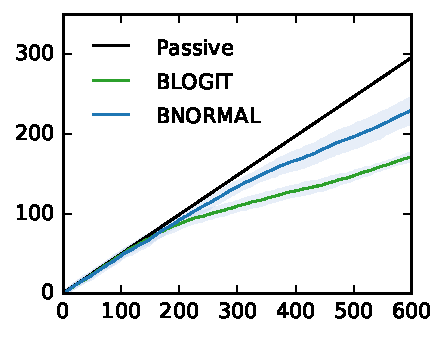
\includegraphics[width=0.42\linewidth]{images/toy_logit_vs_normal_10_10_5.pdf}
	}
	\subfigure[N=20, K=10, D=5\label{fig:syn2}]{
	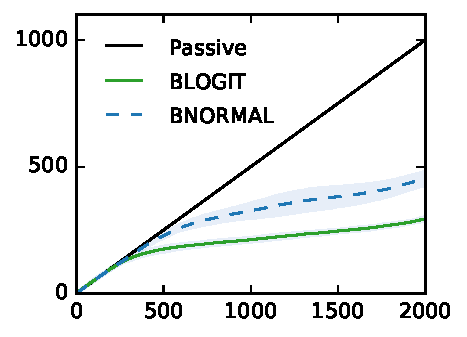
\includegraphics[width=0.445\linewidth]{images/toy_logit_vs_normal_20_10_5.pdf}
	}
	\subfigure[N=5, K=5, D=5\label{fig:syn3}]{
	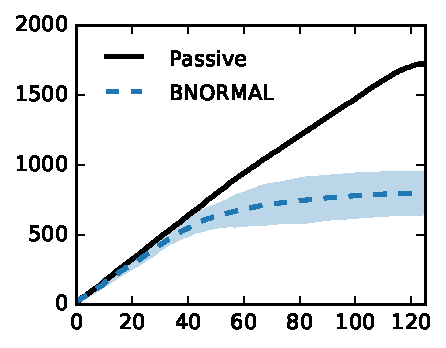
\includegraphics[width=0.42\linewidth]{images/toy_5_5_5.pdf}
	}	
	\subfigure[N=10, K=10, D=5\label{fig:syn4}]{
	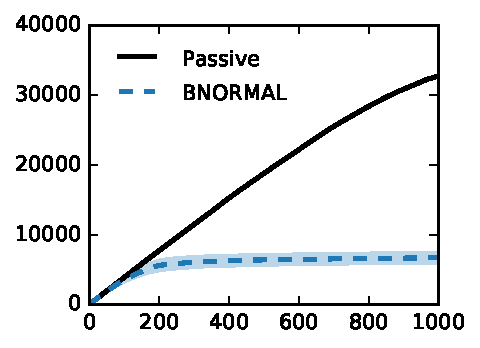
\includegraphics[width=0.45\linewidth]{images/toy_10_10_5.pdf}				
	}
%	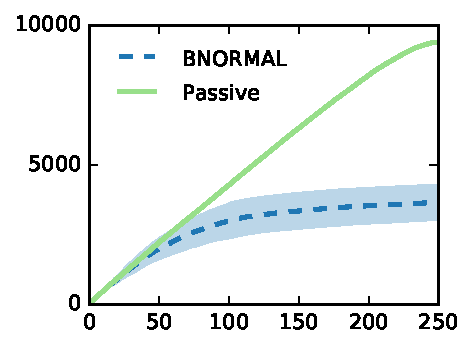
\includegraphics[width=0.32\linewidth]{images/toy_5_10_5.pdf}			
%	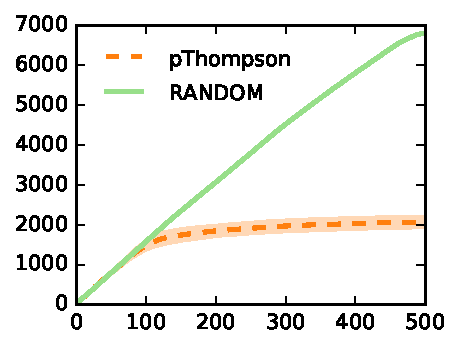
\includegraphics[width=0.32\linewidth]{images/toy_10_5_5.pdf}				
	\caption{\label{fig:synthetic} Cumulative regret of particle Thompson sampling 
	on different sizes of the synthetic dataset. 
	(a, b) Synthetic dataset with logistic output variable.
	(c, d) Synthetic dataset with Gaussian output variable.
	We compared the particle Thompson sampling with passive sampling method. 
	The averaged cumulative regrets are plotted with one standard error. 
	As the model obtained more and more labeled samples from Thompson sampling, 
	the cumulative regrets sub-linearly increase.}
\end{figure}

To verify the particle Thompson sampling, we first synthesise two sets of datasets based on the model assumptions and run 
the Thompson sampling algorithm. By following the model assumptions in Eq. \ref{eqn:entity_gen} to 
\ref{eqn:triple_gen}, we randomly generate triples based on randomly sampled entities and relations. Every 
entities and relations are generated from zero-mean isotropic multivariate normal distribution, where we set 
the variance parameters $\sigma_e$, $\sigma_r$, respectively.
For the final output triple, we generate two sets of datasets with the logistic output variable and the Gaussian output variable. 
The variance of gaussian $\sigma_x$ set to 0.1.

To measure the performance on synthetic dataset, we compute the cumulative regret of proposed algorithm at 
each time $n$ as follows:
\begin{align}
R(n) = \sum_{t=1}^{n} x_t - x^{*}_t,
\end{align}
where $x^*_t$ is the highest triple among triples that have not been chosen up to time $t$. Unlike the general 
Bandit setting where one can select a single item multiple times, in our formulation, we can select one triple 
only once. So after selecting a triple at time $t$, the selected triple will be removed from a set of candidate 
triples.

Figure \ref{fig:synthetic} shows the cumulative regret of the algorithm on the synthetic data with varying size of 
entities and relations. We compare the cumulative regret of the particle Thompson sampling with the passive 
learning method where the model choose a random triple at each time. All results are averaged over 10 
individual runs with different initialisations. 
Note that the dataset with the logistic output variables can be used to train both Bayesian logistic RESCAL (BLOGIT) and Bayesian Gaussian RESCAL (BNORMAL) whereas the dataset with the Gaussian output can only be trained by BNORMAL.
Figure \ref{fig:syn1} and \ref{fig:syn2} show that with the logistic synthetic dataset both models are capable to learn the latent features of the generated triples. 
Figure \ref{fig:syn3} and \ref{fig:syn4} also reveal the capability of BNORMAL with respect to the real valued dataset.
%For every experiment, the cumulative regret of the Thompson 
%sampling method was bounded after a certain number of interactions whereas the cumulative regret of 
%passive learning increases linearly. 
Both results indicate the particle sampling is capable of inferring latent features 
of entities and relations as the interaction increases.

\subsection{Thompson sampling on real datasets}
\begin{table}[t]
\centering
\caption{\label{tbl:dataset}Description of datasets. 
Sparsity denotes the ration of valid triples to invalid triples.}
\vskip 0.15in
\begin{tabular}{l | r | r | r | r}
Dataset &  \# rel & \# entities & \# triples & sparsity \\ \hline
Kinship & 26 & 104  & 10,790 & 0.038 \\
UMLS & 49 &135  & 6,752 & 0.008 \\
Nation & 56 & 14  & 2,024 & 0.184 \\
%Wordnet & 11 & 38,696  &123,429 & 7.5e-06\\
%Wordnet(N) & 10 & 836 & 1,766 & 2.5e-04\\
\end{tabular}
\end{table}

Next, we evaluate our algorithms on real datasets and compare the performance to the various baseline 
algorithms. We use three relational datasets: KINSHIP, UMLS, and NATION. Detailed description of each 
dataset is shown in Table \ref{tbl:dataset} \footnote{https://alchemy.cs.washington.edu/papers/kok07/}.

\textbf{Experimental settings}: 
We compare our model with AMDC, and passive learning with BRESCAL.  
AMDC model has been proposed to achieve two different active learning goals, constructing a predictive
model and maximising the valid triples in a knowledge base, with two different querying strategies
 \cite{kajino2015active}. 
AMDC-PRED is a predictive model construction strategy and chooses a triple which is the most ambiguous triples (close to the decision boundary) at each time $t$.
AMDC-POP is a population strategy which aims to maximise the number of valid triples in a knowledge base. AMDC-POP chooses a triple that has the highest expected value at each time.  
To train all models we only use the observed triples up to the current time. For the passive learning with BRESCAL, we generate a random sample at each time period.
For the particle Thompson sampling, we set both variance parameter $\sigma_e$ and $\sigma_r$ to 1, and $
\sigma_x$ to 0.1. 

We leave 30 \% of triples as a test set to measure test error. 
At each time period, each model choose one triples to query, 
if the selected triple is in the test set then we choose the next highest expected triple which is not in the test set.
All models start from zero observation. 
After every querying, the system obtains a label of the queried triples from an oracle,
then the system updates the parameters of the model. 

\textbf{Evaluation metric}: We use two different evaluation metrics, ROC-AUC score, and cumulative gain,
for the performance comparison. One goal of the Thompson sampling is to maximise the knowledge 
acquisition through the balanced querying strategy between exploration and exploitation. 
To measure how much knowledge are obtained through the querying stage, we fist compute the cumulative 
gain which is the number of obtained valid triple up to time $t$, and then compute the ROC-AUC score on 
test set to understand how this balanced querying strategy results in making a predictive model.

\begin{figure}[t]
	\centering
	
	\subfigure[KINSHIP]{
	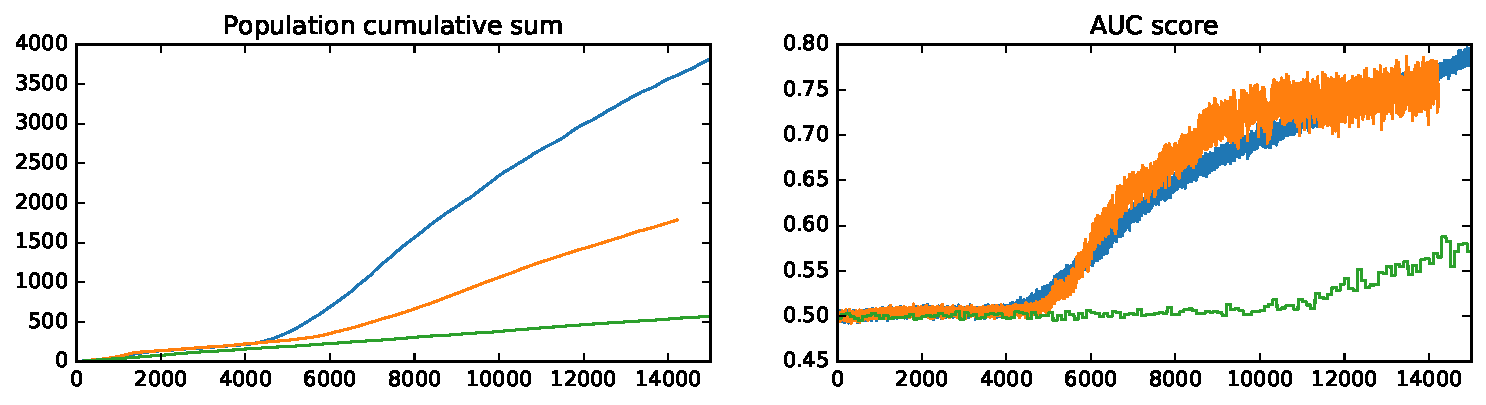
\includegraphics[width=\linewidth]{images/thompson_kinship.pdf}
	}
	\subfigure[UMLS]{
	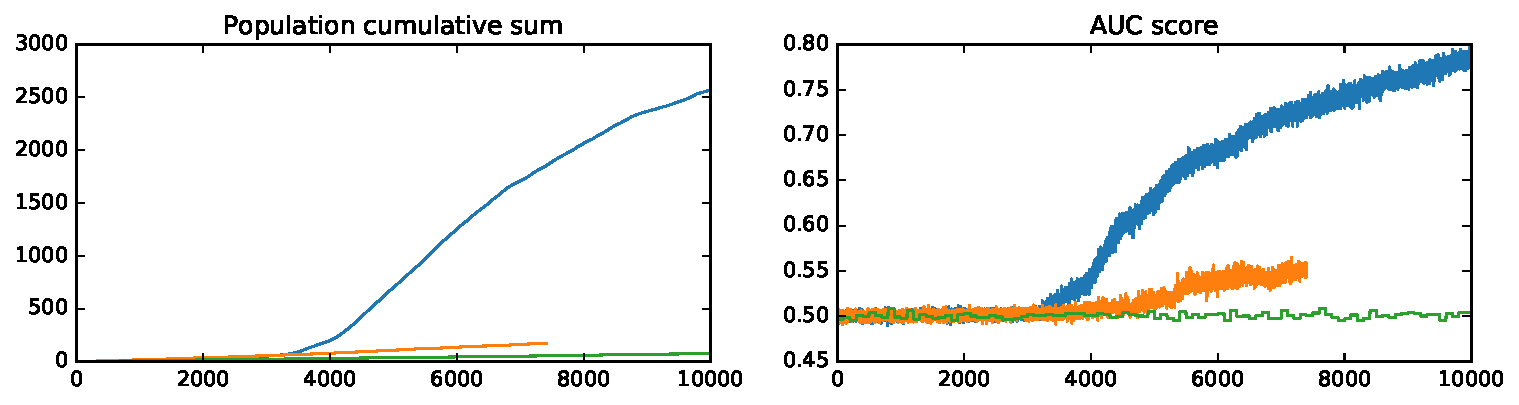
\includegraphics[width=\linewidth]{images/thompson_umls.pdf}				
	}
	\subfigure[NATION]{
	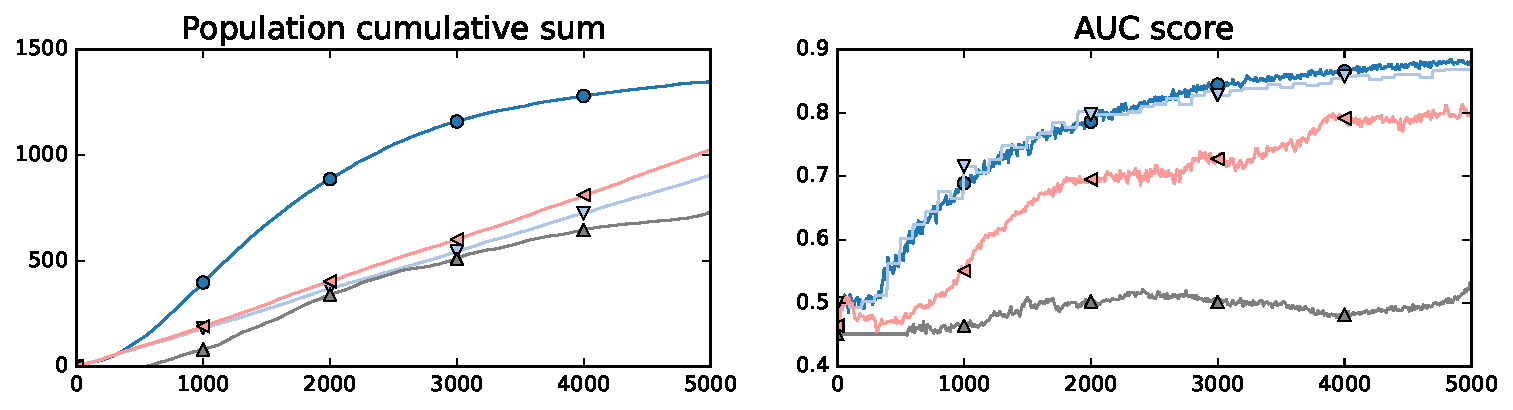
\includegraphics[width=\linewidth]{images/thompson_nation.pdf}				
	}	
	\caption{\label{fig:c_gain}The cumulative gain and ROC-AUC score of the Thompson sampling 
	with various baseline approaches. Thompson sampling with Bayesian RESCAL (BNORMAL)
	model achieves the highest cumulative gain to compare with other active and 
	passive learning algorithms and shows comparable performance on ROC-AUC scores.}
\end{figure}

\textbf{Exploitation and exploration}: 
Figure \ref{fig:c_gain} shows 
the cumulative gain and ROC-AUC scores of the Thompson sampling on three real datasets.
BNORMAL performs better than other baseline models for the cumulative gain, and shows comparable result for the ROC-AUC scores.

In the original AMDC work \cite{kajino2015active}, AMDC-POP model obtains more 
valid triples than AMDC-PRED, and AMDC-PRED shows high ROC-AUC scores than AMDC-POP. 
In our experiment, however, AMDC-POP shows comparable cumulative gain to AMDC-PRED 
and even worse than AMDC-PRED for the UMLS. We conjecture the initial observation 
results in the  different performances: in the original experiment, the model starts
from a small set of training data so the model can exploit a certain latent structure 
given an initially trained model, whereas in our experiment, we start from zero 
observation which makes the model hard to exploit the structure. This result shows 
the importance of balancing between exploitation and exploration.

\subsection{Training with compositional relations}
Applying Thompson sampling to the compositional models is not straight forward. 
Because, in the compositional model, adding one valid triple in a knowledge base will 
change the accompanying compositional paths over the extended tensor $\mathcal{X}^L$. 
Therefore, the system requires to compute potential gains in the 
compositional structure for every candidate query triple. This computational complexity 
will increase exponentially as we increase the length of the composition.

In this experiment, instead running the Thompson sampling for the compositional models,
we follow the standard train/validation/test approach to measure the performance of the compositional models, since the computational complexity of the standard MCMC for the compositional models is endurable. 
The results between active acquisition and training and testing are not always coincident, but if the Thompson sampling samples latent features from true posterior of the compositional model, the samples corresponds to the true posterior samples from the training set.

For all experiments, we set the compositional length $L$ to 2, split datasets into 20\% of validation set and 30\% of test set. We vary the proportion of training triples
from 1\% to 13\% of datasets. Based on the trained model, we measure the ROC-AUC scores on the test set.

Figure \ref{fig:r_vs_br} shows the ROC-AUC scores of the compositional models with the various baseline models. We compare the compositional model with original RESCAL, BNORMAL, and BLOGIT. In general, the multiplicative compositional model (BCOMP\_MUL) outperforms the additive compositional model (BCOMP\_ADD), and outperforms the other baseline models when the proportion of training set is relatively small. For UMLS and NATION, BCOMP\_MUL outperforms across the all training proportions, however for KINSHIP, the model performs better when the training proportion is less than 7\%.

\begin{figure}[t]
	\centering
	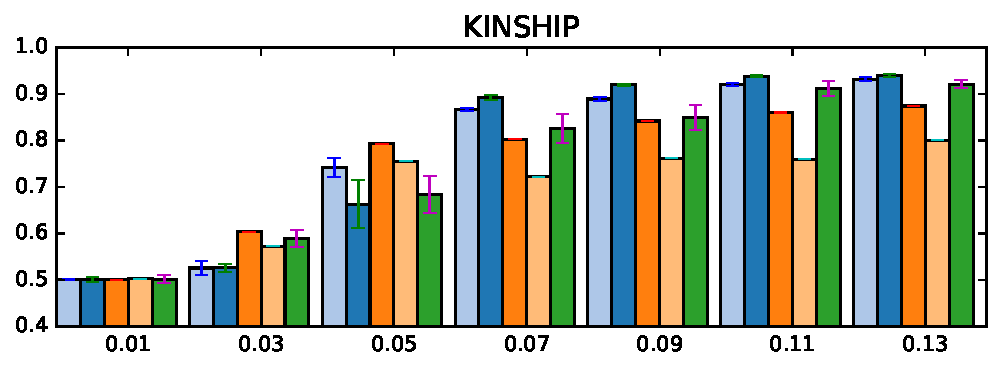
\includegraphics[width=\linewidth]{images/comp_training_error_kinship_small.pdf}
	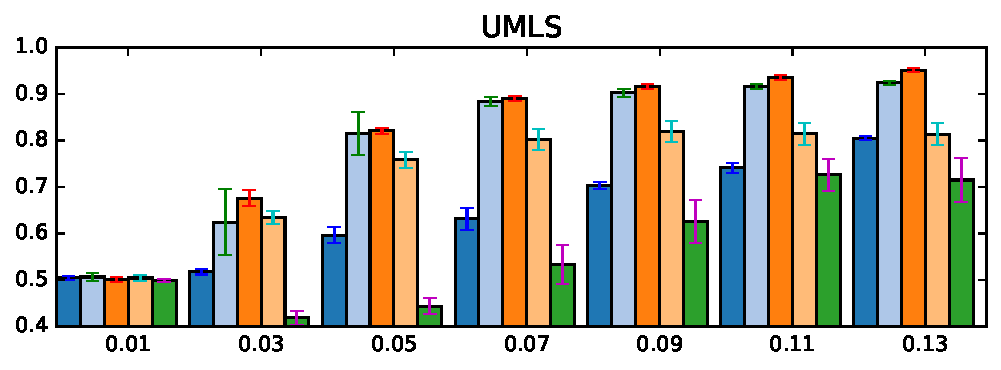
\includegraphics[width=\linewidth]{images/comp_training_error_umls_small.pdf}			
	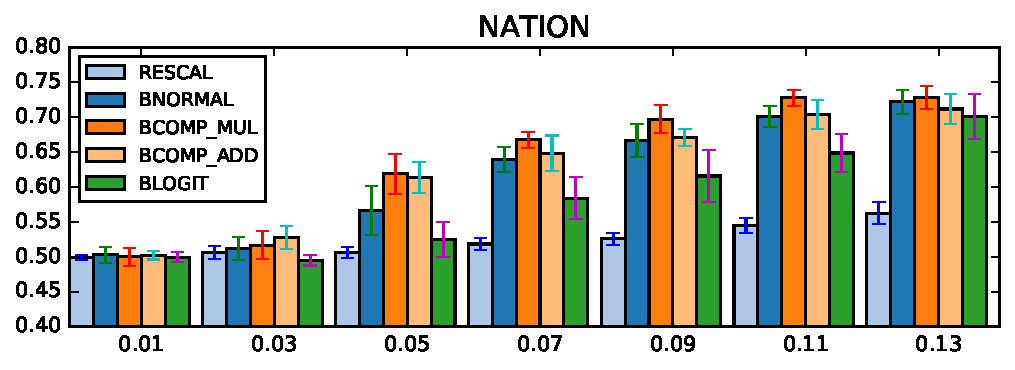
\includegraphics[width=\linewidth]{images/comp_training_error_nation_small.pdf}				
	\caption{\label{fig:r_vs_br} ROC-AUC scores of compositional models. 
	The x-axis denotes the proportion of an observed triples including negative triples used for training 
	models. We use other 20\% of triples as a validation set and another 30\% of triples as a test set. 
%waiting result now...
%In general, compositional models outperform BRESCAL and BLOGIT model when the size of training set is 
%relatively small, whereas BRESCAL and BLOGIT perform slightly better than or comparable to the 
%compositional models when the size of training set is relatively large. For UMLS dataset, the multiplicative 
%compositional model consistently outperforms the other models across all training proportions.
}
\end{figure} 

